% 本章（ch09）原书节号用阿拉伯数字（1, 2, 3, 4 …），与全书多数章用罗马数字不同；
% 按体例在 \chapter 之前切换编号，章末 reflist 之后还原，以免影响后续各章。
\renewcommand{\thesection}{\arabic{section}}

\chapter{镜像对称与 D-模}
\chapterauthor{Martin Guest}{[首都大学東京大学院理工学研究科]}
\chapterauthor{乙藤隆史}{[日本大学工学部]}
% ===== PDF p.117 (原书 p.109) =====
\section{引言}

正如前面各章所讲解的，镜像对称与数学、物理的方方面面都有联系。这次我想说明的是：镜像对称的数学特征中重要的一部分，可以从常微分方程中提取出来。

常微分方程在数学和物理中都是人们熟悉的东西。例如，表示指数函数增长的方程 $y'=ky$（解为 $y=Ae^{kx}$），或者简谐振动的方程 $y''=-ky$（解为 $y=A\sin\sqrt{k}\,x+B\cos\sqrt{k}\,x$），到处都能遇到。微分方程竟成了通往镜像对称的线索——这个话题既有趣又困难，实在出人意料。

当然，镜像对称中出现的微分方程是特殊类型的，研究者们并不容易发现它们。此外，考察这些微分方程时，方便的做法是（在微分几何上）把它们看作平坦联络，或者（在代数上）使用 D-模这一高级工具。下面我们避开技术细节，简要说明这些要点。

“镜像对称与 D-模”这一题目背后的想法是：让镜像对称的微分方程在下面两个完全不同的对象之间充当媒介。这两个对象，一个是与 Gromov--Witten 不变量、辛拓扑相关的量子上同调，另一个是复代数几何中变动的 Hodge 结构。迄今为止，这类意想不到的关联在数学中总是带来极其丰硕的成果。镜像对称的情形也不例外。
% ===== PDF p.118 (原书 p.110) =====
\section{微分方程}

本章只考察 2 阶线性常微分方程。2 阶线性常微分方程是指
\[
y''+a_1(z)y'+a_0(z)y=0
\]
其中 $y=y(z)$ 是复变量 $z$ 的复值函数，$a_0,a_1$ 是给定的复值函数。（如果实数变量的实值函数更容易理解，也可以那样假定来读；但要更深入地理解，复数不可或缺。）

系数 $a_0,a_1$ 为常数时，通解容易表示。例如，若多项式 $t^2+a_1t+a_0$ 有两个不同的根 $\alpha,\beta$，则通解为 $y=Ae^{\alpha z}+Be^{\beta z}$。

系数 $a_0,a_1$ 不是常数时，一般没有表示通解的简单公式；但只要在某点 $z_0$ 处 $a_0,a_1$ 有定义，解在 $z_0$ 附近就存在，而且这样的解的全体构成 2 维向量空间。解通常可以写成 Taylor 级数的形式，必要时当然也可以计算其数值。

当 $a_0,a_1$ 之一在 $z_0$ 处有奇点时，一般找不到在 $z_0$ 处有定义的解，但存在在 $z_0$ 的“附近”有定义的解，可以研究解在接近奇点时如何变化。

例如考察超几何微分方程
\[
y''+\frac{(a+b+1)z-c}{z(z-1)}y'+\frac{ab}{z(z-1)}y=0 \tag{$*$}
\]
（其中 $a,b,c$ 为常数）。该方程在 $z=0,1$ 和 $z=\infty$ 处有奇点（$z=\infty$ 是奇点这一点，通过新变量 $w=1/z$ 改写方程即可看出）。此例以具有许多特殊性质而闻名。例如，当 $c$ 为负整数但非零时，尽管 $z=0$ 是方程的奇点，但在其邻域内存在正则的特解
\[
y=1+\frac{ab}{c}z+\frac{a(a+1)b(b+1)}{c(c+1)}\frac{z^2}{2!}+\cdots
\]
而且，三个奇点都是“正则”奇点，
% ===== PDF p.119 (原书 p.111) =====
这些正则奇点处的行为决定了超几何微分方程的全部性质。当然，要实际描述解的各种行为是极其复杂的；如果正则奇点更多，或者存在非正则奇点，就会越发复杂。

\section{D-模}

2 阶标量方程 $y''+a_1y'+a_0y=0$ 可以变换为 1 阶矩阵方程
\[
\begin{pmatrix}y_0<本地路径>'=
\begin{pmatrix}0&1\\-a_0&-a_1\end{pmatrix}
\begin{pmatrix}y_0<本地路径>,\qquad
\begin{pmatrix}y_0<本地路径>
\begin{pmatrix}y\\y'\end{pmatrix}.
\]
这样做有方便之处。变换的方法不止一种，例如也可以取
\[
\begin{pmatrix}y_0<本地路径>'=
\begin{pmatrix}0&\frac{1}{z}\\-za_0&\frac{1}{z}-a_1\end{pmatrix}
\begin{pmatrix}y_0<本地路径>,\qquad
\begin{pmatrix}y_0<本地路径>
\begin{pmatrix}y\\zy'\end{pmatrix}.
\]

反过来，关于 $y_0,y_1$ 的 1 阶矩阵方程，可以用各种方法变换为关于 $y$ 的 2 阶标量方程。上面的例子中取 $y=y_0$，但也有其他选择（例如取 $y=y_1$，或者把含 $y_0,y_1$ 的式子取作 $y$）。从标量方程到矩阵方程的变换（及其逆）中的这种自由度很重要。正是因为有这种自由度，才能针对给定的问题寻找最合适的最简形式。

若用 D-模的语言来叙述现在我们处理的对象，就得到
\[
\mathcal{M}=\frac{D_z}{(T)}=\frac{\text{所有微分算子}}{\text{由 }T\text{ 生成的左理想}}
\]
这样一个 D-模。这里 $T$ 是微分算子 $\partial_z^2+a_1\partial_z+a_0$，$\partial_z$ 是 $\partial/\partial z$ 的简写。我们不是去考虑微分方程 $Ty=0$，而是考虑 $D_z/(T)$ 这个模。这好比代数几何中不考虑方程 $f(x_1,\cdots,x_n)=0$、而考虑环
\[
A=\frac{\C[x_1,\cdots,x_n]}{(f(x_1,\cdots,x_n))}
\]
的做法。
% ===== PDF p.120 (原书 p.112) =====
把 $A$ 当作抽象的环来看，坐标变换就已经被吸收进定义里了（这是现代数学中常用的想法）。

顺便一提，满足原方程 $f(x_1,\cdots,x_n)=0$ 的点，对应于从环 $A$ 到 $\C$ 的环同态。在 D-模的情形，微分方程 $Ty=0$ 的解，对应于从 $\mathcal{M}$ 到所考虑的函数空间的 $D_z$-同态（详见文献 [5]）。

现在，若选取构成 $\mathcal{M}$ 的基底（在由 $z$ 的函数构成的环上）的微分算子 $P_0,P_1$，就确定了与原标量方程 $Ty=0$ 等价的矩阵微分方程。上面的第一个例子相当于取基底 $1,\partial_z$，第二个例子相当于取 $1,z\partial_z$。方程中的矩阵，就是 $\partial_z$ 作用在 $\mathcal{M}$ 上相对于基底 $P_0,P_1$ 的矩阵。因此，寻找简单矩阵的问题，可以改述为求 D-模的适当基底的问题。这与线性代数中求矩阵标准形的问题十分相似。实际上，Jordan 标准形最早的应用之一，正是这类微分方程的问题（参见 [2] 第 2.4 节）。关于把常微分方程看作 D-模的观点，文献 [4][5] 可供参考。

作为例子，让我们考虑把微分算子
\[
\partial_z^{n+1}+a_n\partial_z^n+\cdots+a_1\partial_z+a_0
=(\partial_z+b_n)(\partial_z+b_{n-1})\cdots(\partial_z+b_0)
\]
作因式分解的问题（这个例子后面会用到）。它类似于多项式的因式分解，但在微分算子环这个非交换的领域里，情况很复杂。利用微分方程的解，可以像下面这样作分解。首先，选取满足初始条件 $u_i^{(j)}(z_0)=\delta_{ij}$ 的解 $u_0,\cdots,u_n$。这些解由初始条件唯一确定。
\[
F=
\begin{pmatrix}
u_0&u_0'&\cdots&u_0^{(n)}\\
\vdots&\vdots&&\vdots\\
u_n&u_n'&\cdots&u_n^{(n)}
\end{pmatrix}
\]
称为基本解矩阵。由定义，$F$ 满足如下等式：
% ===== PDF p.121 (原书 p.113) =====
\[
F^{-1}F'=
\begin{pmatrix}
0&&&-a_0\\
1&\ddots&&\vdots\\
&\ddots&0&-a_{n-1}\\
&&1&-a_n
\end{pmatrix}
\]

这里，施行 Gauss 分解 $F=F_-F_+$（其中 $F_-$ 是对角元为 1 的下三角矩阵，$F_+$ 是上三角矩阵）。于是可知
\[
F_-^{-1}F_-'=
\begin{pmatrix}
0&&&\\
v_1&0&&\\
&v_2&0&\\
&&\ddots&\ddots\\
&&&v_n&0
\end{pmatrix}
\]
这里，函数 $v_0,\cdots,v_n$ 是由条件 $v_0(z_0)=\cdots=v_n(z_0)=1$ 与
\[
u_0=v_0,\qquad
u_1=v_0\!\int\! v_1,\qquad
u_2=v_0\!\int\!\Bigl(v_1\!\int\! v_2\Bigr),\qquad\cdots
\]
从 $u_0,\cdots,u_n$ 唯一确定的函数。

变换 $F\mapsto F_-$ 对应于 D-模的基底变换。而且（由上面的矩阵可知）变换后的算子为
\[
v_0v_1\cdots v_n\,\partial_z\frac{1}{v_n}\cdots\partial_z\frac{1}{v_1}\partial_z\frac{1}{v_0}
\]
（这是常微分方程理论中的 Frobenius 分解）。由于 $\partial_z\frac{1}{v}=\frac{1}{v}\partial_z+\bigl(\frac{1}{v}\bigr)'$，这也意味着原微分方程被分解为一次因子的乘积。要具体执行这个分解，需要先解出微分方程；但正如后面会看到的，能够作这样的分解这一事实本身很有用。用 D-模的语言来说，这个分解对应于子 D-模链 $\mathcal{M}_1\subset\mathcal{M}_2\subset\cdots\subset\mathcal{M}_{n+1}=\mathcal{M}$。
% [Tutor Note: 此处原文作「記号的分解」，译文按中文文献通行的「Frobenius 分解」译出。]

\section{以二维环面为例}

让我们用二维环面 $T^2$ 这个非常简单的例子来说明镜像对称这一现象。说实话，这个例子过于简单，镜像对称最有趣的许多侧面都不会出现。不过，就说明微分方程所起作用这一目的而言，它是一个麻烦较少的好例子。

二维环面是两个圆周的积 $S^1\times S^1$。它可以嵌入三维欧几里得空间，
% ===== PDF p.122 (原书 p.114) =====
\begin{figure}[t]
\centering
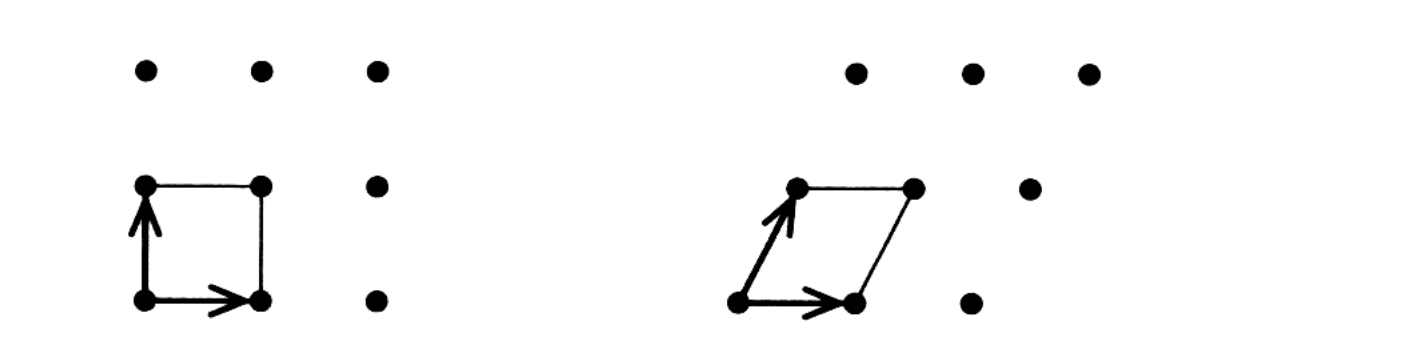
\includegraphics[width=\linewidth]{figures/ch09-fig1.png}
\figtitle{1}{两个不同的格（原书 p.114）}
\end{figure}

通常被画成“有一个洞”的曲面。不过，正如接下来要说明的，观察环面的方法还有别的；（非常粗略地说）那些方法分别体现了镜像对称的两侧。

首先，是把 $T^2$ 看成复平面 $\C$ 用格（lattice）$\Lambda$ 取商所得的商空间 $\C/\Lambda$ 的方法。$\Lambda=\Z\oplus\sqrt{-1}\Z$ 就是格的一个例子；此时环面为 $T^2=S^1\times S^1$。但并不只有这一种。格由 $\C$ 内任意两个在 $\R$ 上一次独立的向量决定，因此按选取方式的不同会得到各种环面。其中每一个都是复李群。

其次，是把 $T^2$ 表示为复射影平面 $\CP^2$ 内的（无奇点的）子流形的方法。这同样有各种表示方式。例如，形如 $z_2^2=z_1^3+az_1+b$ 的方程都确定 $\C^2$ 内的一条复曲线；只要 $4a^3+27b^2\neq0$，再添上无穷远点，就确定了 $\CP^2$ 内的一个环面。换个说法，它是用射影坐标、由 3 次齐次多项式定义的复曲线。这样便得到 $\CP^2$ 内“椭圆曲线”即“3 次超曲面”的族。不把环面单独看待、而是作为族来处理，这在后面会变得重要。

现在，这种情况下应当使用的微分算子，实际上是
\[
\delta^2-3z(3\delta+2)(3\delta+1)
\]
这里 $\delta$ 表示 $z\frac{\partial}{\partial z}$。整理后，得到微分方程
\[
\bigl((1-27z)\delta^2-27z\delta-6z\bigr)y=0 .
\]
奇点是 $0,\frac{1}{27},\infty$ 这 3 点。用 Frobenius 方法可以求出 $z=0$ 附近的解的级数展开，得到如下形式的线性无关解：
\[
u_0=f_0,\qquad u_1=f_0\log z+f_1 .
\]
% [Tutor Note: $\CP^2$ 内“3 次超曲面”是余维 1 的对象，即一条 3 次曲线；原书沿用“超曲面”的称呼，译文照录。]

% ===== PDF p.123 (原书 p.115) =====
其中 $f_0,f_1$ 在 $z=0$ 处全纯，且满足 $f_0(0)=1$，$f_1(0)=0$。级数展开的开头几项为
\[
f_0(z)=1+6z+90z^2+\cdots
\]
\[
f_1(z)=15z+\frac{513}{2}z^2+\cdots
\]
这里只写出开头几项。

这个常微分方程是超几何微分方程的一例；把 $z$ 换成 $z/27$，它就化为第 2 节所列的式 (∗) 中取 $a=\frac{1}{3}$，$b=\frac{2}{3}$，$c=1$ 的情形。即使在超几何微分方程的族中，这个解的行为也很特殊。正如后面会看到的，这不过是冰山一角。

关于微分算子 $\delta^2-3z(3\delta+2)(3\delta+1)$ 的来历，我不做详细说明，只提一句：其背后有一套一贯的理论（GKZ 方程与环簇的理论）支配着这一切。例如，$\CP^{N-1}$ 内次数 $k$ 的非奇异超曲面所对应的微分算子是
\[
\delta^{N-1}-kz(k\delta+k-1)\cdots(k\delta+1) .
\]
$k=N=5$ 的情形，就是把镜像对称引入数学的著名例子——4 维射影空间内 5 次超曲面对应的微分算子。

\section{提取 Gromov--Witten 不变量（量子上同调）}

在量子上同调中 D-模所起的作用，是由 Givental [1] 揭示的。简单说来，Givental 的见解是：所谓“量子 D-模”这种 D-模，是比量子上同调环更为基本的对象。

复射影空间 $\CP^n$ 的量子上同调环表示为
\[
QH^*\CP^n=\frac{\C[x,q]}{(x^{n+1}-q)} .
\]
此外，复射影空间 $\CP^n$ 的量子 D-模为
\[
\mathcal{M}_{\CP^n}=\frac{D_t}{(\partial_t^{n+1}-q)} .
\]
其中取 $q=e^t$。另外，$D_t$ 是由 $\partial_t=q\partial_q$ 生成的微分算子所成的环。（这里用 $t$ 代替了前面使用的变量 $z$，
% ===== PDF p.124 (原书 p.116) =====
通常，在量子上同调中使用的是这个 $t$。）

对于 $\CP^n$ 以外的空间，（交换的）量子上同调环与（非交换的）量子 D-模之间的关系，在大多数情况下要复杂得多。不过，$T^2$ 的情形却变得简单。这是因为全纯映射 $\CP^1\to T^2$ 总是常值映射，所以量子上同调环与通常的上同调环在本质上没有变化。把上同调环、量子上同调环的偶数次部分所构成的子环分别记作 $H^*$ 与 $QH^*$，则
\[
QH^*T^2=H^*T^2\otimes\C[q]=\frac{\C[x,q]}{(x^2)} ,
\]
并且
\[
\mathcal{M}_{T^2}=\frac{D_t}{(\partial_t^2)} .
\]

现在，让我们说明从 D-模
\[
\mathcal{M}=\frac{D_\theta}{\Bigl(\partial_\theta^2-\frac{27z}{1-27z}\partial_\theta-\frac{6z}{1-27z}\Bigr)}
\]
出发，构造这个 $T^2$ 的量子 D-模的步骤（为什么这样做能行得通，说明从略）。这里取 $z=e^{\theta}$。于是 $z\partial_z=\partial_\theta$ 成立。变量 $q,t$ 是 $z,\theta$ 的类似物。实际上，正如后面会看到的，提取 $T^2$ 的量子上同调时，主要的一步是从 $z$ 到 $q$ 的（多少有些不易看出的）坐标变换。

如前所述，我们的常微分方程可以写成因式分解的形式：
\[
(1-27z)v_0v_1\partial_\theta\frac{1}{v_1}\partial_\theta\frac{1}{v_0}
\]
这里 $v_0=u_0$，$v_1=\partial_\theta\frac{u_1}{u_0}$。从这个形式可以看出，当前问题中恰当的坐标变换是什么：取 $\frac{1}{v_1}\partial_\theta=\partial_t$。换个说法，用
\[
t=\int v_1(z)\,d\theta=\frac{u_1(z)}{u_0(z)}=\log z+\frac{f_1(z)}{f_0(z)}=\log z+15z+\frac{333}{2}z^2+\cdots
\]
即
\[
q=ze^{f_1(z)/f_0(z)}=z+15z^2+279z^3+\cdots
\]
来定义新的变量 $t$。这样一来，我们的微分算子就变成
% ===== PDF p.125 (原书 p.117) =====
$\partial_t^2$（乘以某个函数）的形式。由此就得到所求的量子 D-模 $\mathcal{M}_{T^2}$。

到目前为止，关于 Gromov--Witten 不变量我们还什么都没有说明。Gromov--Witten 不变量，就是充当量子上同调环的结构常数的那些量。在 $T^2$ 的情形，它相当于量子积
\[
x\circ x=a\cdot 1+b\,x
\]
中的系数 $a,b$。$T^2$ 的情形不用再做任何计算，由关系式 $x^2=0$ 就直接得到 $a=b=0$。

让我们看看结构常数的这个结果是如何从 D-模 $\mathcal{M}$ 导出的。$T^2$ 的情形如上所见，只用上同调的表示式就能得到结果，不必特意搬出 D-模。但这一手法本身适用于更一般的空间，有时会得出非平凡的结果。把原来的标量微分方程用基底 $1,\partial_\theta$ 变换为矩阵微分方程，就得到
\[
\partial_\theta\begin{pmatrix}y_0<本地路径>
\begin{pmatrix}0&1\\ \frac{6z}{1-27z}&\frac{27z}{1-27z}\end{pmatrix}
\begin{pmatrix}y_0<本地路径> .
\]
使用另一个基底 $\frac{1}{v_0},\frac{1}{v_1}\partial_\theta\frac{1}{v_0}$，则得到下面的形式
\[
\partial_\theta\begin{pmatrix}y_0<本地路径>
\begin{pmatrix}0&v_1\\0&0\end{pmatrix}
\begin{pmatrix}y_0<本地路径> .
\]
最后，通过坐标变换把函数 $v_1$ 变成常数函数 1。结构常数就是由此所得矩阵的系数。也就是说，导出了 $x\circ 1=x$ 与 $x\circ x=0$。

对于 4 维射影空间内的 5 次超曲面，用同样的步骤可以得到形如
\[
\partial_t^2 f\,\partial_t^2
\]
（$f$ 是某个函数）的微分算子。把 $f$ 移到通常的、可交换的函数环中就可以去掉，因此可以看出，量子上同调环具有与通常的上同调环相同的 $x^4$ 关系式。不过，在当前情形中 Gromov--Witten 不变量并没有消失。这是因为，函数 $f$ 在结构常数所构成的 $4\times 4$ 矩阵中存留了下来。
% ===== PDF p.126 (原书 p.118) =====
\section{提取 Hodge 结构}

微分算子 $\delta^2-3z(3\delta+2)(3\delta+1)$ 的因式分解，在镜像对称的另一侧也很重要。正如第 3 节所注意到的，这个因式分解对应于子 D-模 $\mathcal{M}_1\subseteq\mathcal{M}$。这可以解读为：它给出 $\C^2$ 内复直线的族
\[
\mathrm{Span}\left\{\begin{pmatrix}u_0<本地路径>
\subseteq
\mathrm{Span}\left\{\begin{pmatrix}u_0<本地路径>,\begin{pmatrix}u_0'\\u_1'\end{pmatrix}\right\}=\C^2
\]
（本节中 $u'$ 表示 $\partial_\theta u=z\partial_z u=\delta u$。）这条复直线随参数变动，就给出到 $\CP^1$ 的全纯映射。对于 4 维射影空间内的 5 次超曲面，考虑以分量 $u_0,u_1,u_2,u_3$ 为列的向量 $u$，就得到“旗（flag）”
\begin{align*}
\mathrm{Span}\{u\}&\subseteq\mathrm{Span}\{u,u'\}\\
&\subseteq\mathrm{Span}\{u,u',u''\}\\
&\subseteq\mathrm{Span}\{u,u',u'',u'''\}=\C^4 .
\end{align*}
实际上，这还有别的几何意义：它正是“变动的 Hodge 结构（VHS）的周期映射”。对我们这个微分方程的“量子上同调”解释，是比较近期（1990 年代）物理学中的发现；而作为 VHS 的解释则更早就有，来自复流形的几何学（1970 年代）。

基本想法是：对先前出现的、构成族的环面，考察它们的上同调群，就能看出这一点。首先，众所周知上同调群 $H^1(T^2,\Z)$ 是 $\Z\oplus\Z$（也就是由两条基本 1-闭链生成）。因此，向量空间 $H^1(T^2,\C)$ 是 $\C^2$（用 de Rham 上同调的语言来说，就是可以取到两个一次独立的 1-形式 $dx,dy$）。这与在哪个环面上考虑无关。也就是说，环面在拓扑上彼此都等价，具有相同的上同调。不过，对复流形还可以考虑 $(p,q)$-上同调。它是由含 $p$ 个 $dz$ 与 $q$ 个 $d\bar z$ 的 $(p+q)$-形式构成的。它显然依赖于复结构。而各种环面的复结构大体上互不相同。因此，
% [Tutor Note: VHS 是 variation of Hodge structure（变动的 Hodge 结构）的缩写。Hodge 数、Hodge 分解这些概念第 1 章与第 4 章已经用过；把它们随参数变动的整体情形一并处理，就叫 VHS。]
% ===== PDF p.127 (原书 p.119) =====
在与 $T^2$ 选取方式无关的 2 维向量空间 $H^1(T^2,\C)$ 内，得到依赖于 $T^2$ 选取方式的子空间 $H^{1,0}(T^2,\C)$。对 5 次超曲面的情形，则得到子空间的“旗”
\begin{align*}
H^{3,0}&\subseteq H^{3,0}\oplus H^{2,1}\\
&\subseteq H^{3,0}\oplus H^{2,1}\oplus H^{1,2}\\
&\subseteq H^{3,0}\oplus H^{2,1}\oplus H^{1,2}\oplus H^{0,3}=H^3 .
\end{align*}
这样确定的从复结构模空间到“旗流形”的映射，就是 VHS 的具体例子。

要看出第 4 节从微分方程得到的映射与这个 VHS 的映射一致，只需看出该微分方程由环面的周期积分所满足即可。函数 $u_1/u_0$ 与著名的模函数 $J$ 的反函数有密切关联。实际上，
\[
J=\frac{1}{1728}\frac{(1+216z)^3}{z(1-27z)^3}
=\frac{1}{1728}\bigl(q^{-1}+744+196884q+\cdots\bigr)
\]
成立。其中 $z=q-15q^2+171q^3-\cdots$（这是把前面出现的级数 $q=z+15z^2+279z^3+\cdots$ 关于 $z$ 解出的结果）。更详细的说明见 [6]。

还有一个尚未说明、重要而微妙的点。第 5 节使用了 $H^0T^2\oplus H^2T^2$，而第 6 节使用了 $H^1T^2=H^{1,0}T^2\oplus H^{0,1}T^2$。一般而言，镜像对称把
（1）$M$ 的量子上同调的某个部分
与
（2）另一个流形 $\widetilde{M}$（“镜像伙伴”）的上同调的另一个部分
对应起来。当 $M=T^2$ 时，$\widetilde{M}$ 也是环面。

\section{结语}

D-模与平坦联络的概念非常接近，所以在讲述镜像对称时，不用 D-模也能对付过去。然而，D-模作为语言是非常方便的，尤其在处理多变量函数时，它的便利性更为突出。为什么在镜像对称中需要 D-模？对这个问题的说明，最有说服力的是：“所谓‘镜像对称的 D-模’，独立于量子上同调和 VHS，其自身就应当作为
% [Tutor Note: 此处的 $J$ 是椭圆曲线模函数 $j$ 的 $1/1728$ 倍；$j=q^{-1}+744+196884q+\cdots$ 是模不变量，书中未加说明。]

% ===== PDF p.128 (原书 p.120) =====
重要的几何对象而存在。量子上同调与 VHS 都只不过是它的具体实现。”通过检验这一想法，就会得到说明吧。刻画出这样的 D-模，是当前研究中一个有趣的课题。

\begin{reflist}
  \item[{[1]}] A. B. Givental, \textit{Homological geometry I, Projective hypersurfaces},
    Selecta Math. \textbf{1} (1995), pp. 325--345.
  \item[{[2]}] ジェレミー·J·グレイ（関口次郎·室政和訳），
    『リーマンからポアンカレにいたる線型微分方程式と群論』，
    シュプリンガー·フェアラーク東京，2002（原書第二版（2000）の訳）．
  \item[{[3]}] M. A. Guest, \textit{From Quantum Cohomology to Integrable Systems},
    Oxford Univ. Press, 2008.
  \item[{[4]}] A. Haefliger, \textit{Local theory of meromorphic connections in dimension one (Fuchs theory)},
    Algebraic D-modules, eds. A. Borel et al., Perspectives in Math. 2, Academic Press, 1987, pp. 129--149.
  \item[{[5]}] 堀田良之，『加群十話』（すうがくぶっくす 3），朝倉書店，1988.
  \item[{[6]}] A. Klemm, B. H. Lian, S. S. Roan, and S. T. Yau,
    \textit{A note on ODEs from mirror symmetry},
    Functional analysis on the eve of the 21st century, volume 2, eds. S. Gindikin et al.,
    Progress in Math. 132, Birkh\"auser, 1996, pp. 301--323.
\end{reflist}

\begin{flushright}
[Martin Guest]
\end{flushright}

% 原书 p.120 末尾的署名有「[Martin Guest]」「[おとふじ たかし]」两行，后者是乙藤隆史姓名的读音标记，
% 按 STYLE_GUIDE §3.7 省略（记入 reports/ch09.md）。

% 本章节号在此还原为罗马数字，恢复全书默认体例（章首曾切换为阿拉伯数字）。
\renewcommand{\thesection}{\Roman{section}}